
\chapter{P\'erdida Esperada}
\noindent Con frecuencia nos enfrentamos a situaciones donde debemos tomar decisiones de trascendencia, tanto de inter\'es personal como de inter\'es organizacional. La importancia  de una decisi\'on depende del riesgo asociado a ella, por lo cual es importante conocer,
tanto su probabilidad, como su costo. El proceso que conlleva una decisi\'on puede realizarse identificando adecuadamente los siguientes aspectos:

\begin{itemize}
\item Localizar el punto en donde se requiere tomar la decisi\'on.
\item Establecer una serie de hip\'otesis que pueden ser aceptadas o refutadas mediante el uso de modelos que se han dise\~nado para tal fin.
\item Conocer las consecuencias asociadas a las diferentes elecciones posibles, las cuales frecuentemente son medidas en costos monetarios.\end{itemize}


%En cualquier entorno de decisi\'on se distinguen los siguientes elementos:
%
%
%\begin{itemize}
%\item Una o mas decisiones que tienen una serie de objetivos y metas definidos.
%\item Un conjunto de acciones o alternativas disponibles para las decisiones.
%\item Un entorno de posibles resultados por la instrumentaci\'on de acciones.
%\item Una funci\'on que asocia acciones y resultados del entorno.
%\item Un proceso de decisi\'on, que selecciona una o varias acciones, dado un cierto entorno.
%\item Un criterio que marca el proceso de decisi\'on.
%
%\end{itemize}

\noindent Uno de los principales objetivos al realizar un estudio de confiabilidad, es tomar decisiones que minimicen costos. El tema de optimizaci\'on no se aborda dentro de la literatura cl\'asica de confiabilidad. Es com\'un que para pronosticar algunas cantidades de inter\'es  se consideren cuantiles adecuados, ya sean bajos o altos, seg\'un el problema que se desee resolver, omitiendo consideraciones externas como monetarias u optimizaci\'on de procesos.

\noindent Lo ideal ser\'ia decidir en forma adecuada, considerando todos los factores y prever de antemano los costos asociados a esa decisi\'on, para as\'i enfocar programas que reflejen una reducci\'on de costos.

\noindent En este trabajo se dise\~na una metodolog\'ia para la construcci\'on de un plan \'optimo de almacenamiento de transformadores. Haciendo uso de una funci\'on de p\'erdida que ser\'a definida en un contexto, que permita minimizar los costos del almac\'en.


\section{Almacenamiento de Transformadores}

\noindent Los transformadores de instrumento son herramientas costosas y dif\'iciles de transportar. La mayor\'ia de las empresas que fabrican este tipo de transformadores lo hacen bajo pedido y se tardan un tiempo considerable en cumplirlo. Su abastecimiento resulta una tarea a optimizar, debido a los costos que pueden minimizarse, como transporte y el costo del almacenamiento mismo, cuando no se usaron los aparatos. Sin embargo esta optimizaci\'on, debe ser tal que no permita que la empresa se quede sin transformadores puesto que esto implicar\'ia un costo  por no poder cobrar el servicio.

\noindent En el presente trabajo se busca desarrollar un plan de inventario para la optimizaci\'on del n\'umero de transformadores almacenados a un tiempo $t$. Para ello necesitamos tener cierta informaci\'on sobre la manera en que debe operar el almac\'en.
%, a continuaci\'on se definir\'an 

%algunas consideraciones importantes.\\[0.2cm]
\noindent Sea $n_0$ el n\'umero inicial de transformadores disponibles para reemplazar a los que fallan. Supongamos que al momento en que falla un transformador, se hace el pedido para sustituirlo y se espera un periodo de $\delta$ meses hasta que llega la orden. Mientras tanto este se reemplazar\'a por uno de los $n_0$ disponibles, si es que todav\'ia quedan en el almac\'en. Interesa determinar el valor de $n_0$, que asegure que a lo largo del periodo de tiempo analizado $(0,t)$, el almac\'en tenga los suficientes transformadores para cubrir las fallas a un costo m\'inimo.\\[0.2cm]
\noindent En el cap\'itulo anterior obtuvimos la muestra de la distribuci\'on posterior para los par\'ametros, que describen el comportamiento del tiempo de vida de los transformadores. La Figura \ref{lo} muestra un esquema representativo, de los elementos disponibles para la construcci\'on de la funci\'on de p\'erdida, que conduzca a la determinaci\'on de $n_0$.
\begin{figure}[h!]
\hspace{-2 cm}
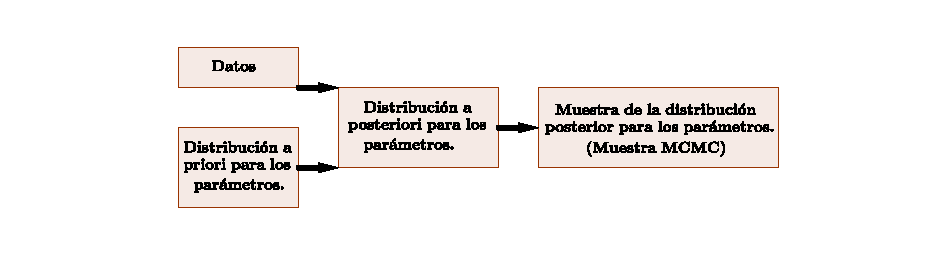
\includegraphics[scale=1.2]{esq.pdf}
\vspace{-1.5cm}\caption{\bf Etapas Realizadas en el Cap\'itulo Anterior.}\label{lo}
\end{figure}
\noindent Mientras que la Figura \ref{op} es un diagrama general de las etapas para  determinar la propuesta de inventario \'optima, empleando  la muestra de la distribuci\'on posterior y algunos costos que posteriormente estableceremos.

\begin{figure}[h!]
\hspace{-1 cm}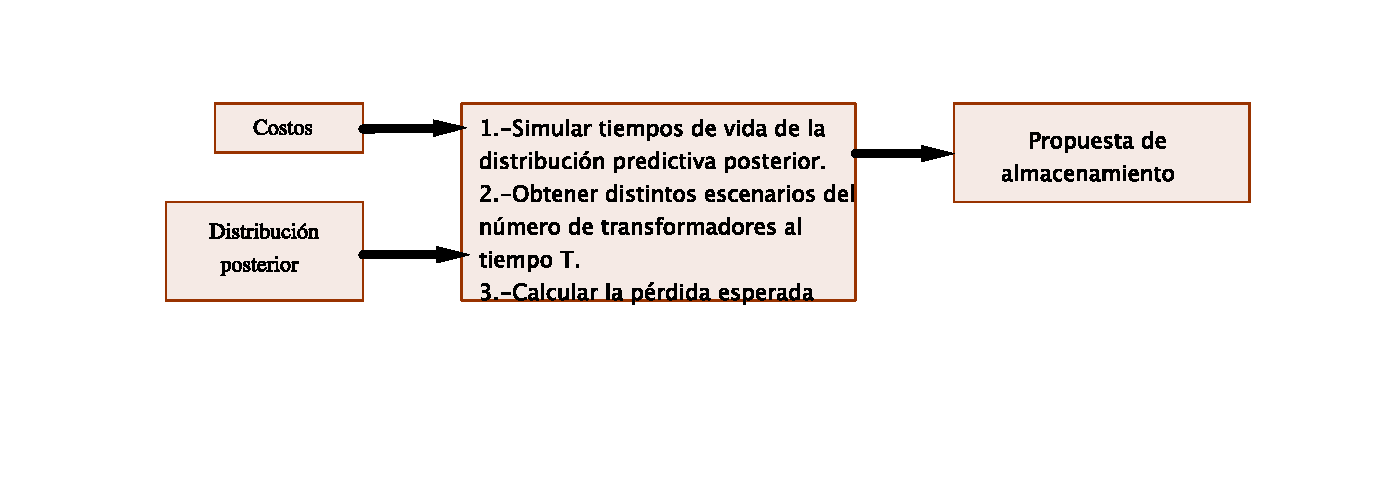
\includegraphics[scale=0.7]{final.pdf}
\vspace{-2.4 cm}\caption{\bf Contrucci\'on del Plan de Almacenamiento.}\label{op}
\end{figure}


\noindent El procedimiento  para determinar el valor \'optimo de $n_0$, se basa en el c\'alculo de la funci\'on de p\'erdida esperada. Para esto simulamos tiempos de vida $t_1,t_2,\cdots, t_n$. El tiempo $t_i$, $i=1,\cdots,n$ provendr\'a de una distribuci\'on Weibull con par\'ametros $(\beta_i,\eta_i)$ de la muestra que ya se obtuvo de la distribuci\'on posterior. Tabla \ref{ejee} contiene un conjunto de realizaciones $(\beta,\eta)$ de la distribuci\'on posterior y el $t_i$ correspondiente,

\begin{itemize}
\item $t_1=274$ es un dato que proviene de la distribuci\'on Weibull(2.228,347.37).
\item $t_2=542$ es un dato que proviene de la distribuci\'on Weibull(2.386,358.77).
\item $t_3=30.5$ es un dato que proviene de la distribuci\'on Weibull(3.534,350.55).
\item $\vdots$
\item $t_n=180$ es un dato que proviene de la distribuci\'on Weibull(2.456,340.51).
\end{itemize}
\noindent Los tiempos de vida simulados pueden ser considerados como una muestra, que resulta de una mezcla de distribuciones Weibull. Se puede demostrar que estos tiempos de vida provienen de la distribuci\'on posterior predictiva de $t$. Se calcula por medio de la siguiente integral:
\begin{eqnarray*}
f(t|\mbox{Datos})&=& \int f(t|\beta,\eta)f(\beta,\eta|\mbox{Datos})d\beta d\eta
\end{eqnarray*}

y se aproxima por medio de (\ref{c}).



\begin{table}
\begin{center}

\vspace{-.3 cm}\caption{\bf Muestra MCMC.}\label{ejee}
\vspace{0.3cm}\begin{tabular}{cccc}
\toprule[0.6mm]
$i$&$\beta$ &$\eta$& $t_i$\\\toprule[0.6mm]
1&2.228 & 347.37 & 274
\\ 2&2.386 & 358.77 & 542
\\3&3.534 & 350.55 &305\\
 $\vdots$&$\vdots$ & $\vdots$ &$\vdots$
\\$n$& 2.456 & 340.51 & 180\\
\toprule[0.6mm]
\end{tabular}
\end{center}

\end{table}
\newpage

%\item {\bf Obtenci\'on de distintos escenarios del n\'umero de transformadores en el almac\'en}

\noindent Una vez establecidos los tiempos de falla de los transformadores. El n\'umero de transformadores en el almac\'en hasta el  tiempo $t$, depender\'a del n\'umero de fallas que ocurran durante el periodo de observaci\'on $(0,t)$, de $\delta$ y del n\'umero de transformadores que fijemos como iniciales $n_0$, es decir, es una funci\'on: $$n(t,n_0,\delta).$$
\noindent Para observar el comportamiento de $n(t,n_0,\delta)$ por simulaci\'on, se consideran tiempos de falla similares a los de la  Tabla \ref{ejee}. Se asume que al momento en que falla un transformador se solicita y llega $\delta$ meses despu\'es. Como solo se pide un transformador cuando alguno ha fallado, siempre tendremos en el almac\'en a lo m\'as $n_0$ transformadores.
\noindent De manera m\'as clara la forma de operar de $n(t,n_0,\delta)$, el n\'umero de transformadores disponibles en el almac\'en en el intervalo de tiempo de  $(0,t)$ es la siguiente: Al inicio del periodo $n(0,n_0,\delta)=n_0$, una vez que se llega a un tiempo de falla $t_1$ el valor de $n(t_1,n_0,\delta)$ ser\'a $n_0-1$ disminuye en uno y este se recuper\'a $\delta$ meses despu\'es. Si se llega a otro tiempo de falla antes de que llegue la orden entonces $n(\cdot)$ disminuir\'a en uno nuevamente, si ocurre lo contrario se recuperar\'a al menos en una unidad.\\[0.1cm]

\noindent Las gr\'aficas de algunas trayectorias simuladas de la funci\'on $n(t,n_0,\delta)$ para valores de $\delta=6,8$ y 12 meses  se muestran en las Figuras \ref{d6} \ref{d8} y \ref{d12}.

 \noindent Se decidi\'o analizar estos valores de $\delta$ , debido a que si los transformadores llegan en periodos menores de 6 meses, los valores de $n(t,n_0,\delta)$ no var\'ian de manera significativa. Por otro lado considerar periodos de espera m\'as largos que un a\~no parece ser un periodo grande de espera. 
\noindent Necesitamos establecer una funci\'on de p\'erdida, a partir de los escenarios simulados,  que permita saber la cantidad inicial adecuada de transformadores que deben tenerse en el almac\'en. La siguiente secci\'on describir\'a la manera de establecer esta funci\'on.


%\end{itemize}
%Rplot06
\begin{figure}
\begin{center}
\includegraphics[scale=.3]{Rplot06.pdf}
\end{center}
\vspace{-1 cm} \caption{\bf Dos trayectorias obtenidas mediante simulaci\'on del n\'umero de transformadores en el almac\'en hasta el tiempo $t=200$ meses,  con $n_0=5$ transformadores al inicio del periodo de observaci\'on y $\delta=6$ meses de espera de llegada de los transformadores que se han pedido.}\label{d6}
\end{figure}
\vspace{-1.5cm}
\begin{figure}
\begin{center}
\includegraphics[scale=.3]{Rplot08.pdf}
\end{center}
\vspace{-1 cm}\caption{\bf Dos trayectorias obtenidas mediantes simulaci\'on del n\'umero de transformadores en el almac\'en hasta el tiempo $t=200$, con $n_0=7$ y $\delta=8$}\label{d8}
\end{figure}

\begin{figure}
\begin{center}
\includegraphics[scale=0.3]{Rplot10.pdf}
\end{center}
\vspace{-1 cm}\caption{\bf Trayectorias simuladas del n\'umero de transformadores en inventario o almacenados con $n_0=10$, $t=200$ y $\delta=12.$}\label{d12}
\end{figure}


\section{Funciones de P\'erdida}

\noindent Al hablar de funci\'on de p\'erdida nos referimos a una funci\'on que expresa los costos de p\'erdidas o ganancias  al tomar diferentes acciones. A continuaci\'on se proponen tres posibles pol\'iticas de inventario y posteriormente se describen sus funciones de p\'erdida. Se considera una pol\'itica de inventario, al planteamiento de una funci\'on de p\'erdida que refleje los costos de mayor inter\'es para la empresa.



\begin{description}
\item [Pol\'itica A] \hfill \\ 
La primera pol\'itica reflejar\'a el costo de quedarnos sin transformadores disponibles en el almac\'en. Estar\'a  enfocada a determinar el $n_0$ adecuado, tal que no permita que dentro del periodo de observaci\'on, el almac\'en se quede sin transformadores para cubrir todas sus demandas.
\item [Pol\'itica B] \hfill \\
La segunda pol\'itica adem\'as de considerar el costo de la pol\'itica A, adiciona el costo del lote inicial de transformadores en el almac\'en. 
\item [Pol\'itica C] \hfill \\
Esta \'ultima pol\'itica se centra en evaluar dos tipos de costos.
\begin{itemize}
\item[1.-] Costo de falta de transformadores por unidad de tiempo. Este costo tambi\'en considerado en las pol\'iticas anteriores.
\item[2.-] Costo de almacenamiento por cada unidad de tiempo.
\end{itemize}
\end{description}

\subsection{Pol\'itica A}

\noindent Usando las Figuras \ref{d6} \ref{d8} y \ref{d12}, es posible obtener la permanencia por debajo de cero de las trayectorias para distintos valores iniciales de $n_0$, lo cual se interpretar\'ia como el n\'umero de veces que la empresa se quedo sin transformadores para reemplazar. Es natural que entre m\'as peque\~no sea $n_0$, se permanece m\'as tiempo por debajo de cero y entre m\'as grande, la empresa se quedar\'a sin reservas por menos tiempo.\\[0.1cm]
\noindent Supongamos que se tiene una trayectoria como la de la Figura \ref{tr}, hasta un tiempo de $10$ meses y con $1$ transformador inicial de reserva. Supongamos adem\'as que al tiempo 3 falla un transformador, luego  $n(3)=0$. Despu\'es de un tiempo falla otro y no tenemos repuesto, entonces el n\'umero de transformadores en reserva es negativo ($n(4)=-1$). La p\'erdida asociada a partir de este tiempo, es el n\'umero de meses que permanece en esta situaci\'on (1 mes), multiplicada por un valor de $c$ unidades monetarias, que representa el costo de no poder cobrar la electricidad, por cada mes que no se tuvo un transformador de instrumento. Si se observa hasta $t=10$ entonces habr\'ia que sumar las p\'erdidas que representan el segundo bloque, que empieza en el tiempo $t=6$. Del bloque de $t=6$ a $t=7$ la p\'erdida involucra solamente a un transformador. Sin embargo en el intervalo de tiempo de $[7,9]$ meses la p\'erdida es m\'as grande, puesto que faltan dos transformadores para sustituir. La p\'erdida  ser\'a  los dos transformadores faltantes multiplicada por la longitud de tiempo que dure este hecho, (2 meses) por el valor de $c$. Por lo tanto la p\'erdida  total es:
\begin{eqnarray*}
c[1\cdot1 + 1\cdot1+2\cdot2+1\cdot1]
\end{eqnarray*} 
Lo que significa que la p\'erdida es la suma de las \'areas delimitadas por debajo de cero, multiplicada por $c$, donde $c$ se tiene que establecer con informaci\'on adicional. Sin perder generalidad se puede suponer $c=1$.\\[0.2cm]

\begin{figure}[h!]
\begin{center}
%\includegraphics[width=10cm,height=5cm]{Rplot01.png}
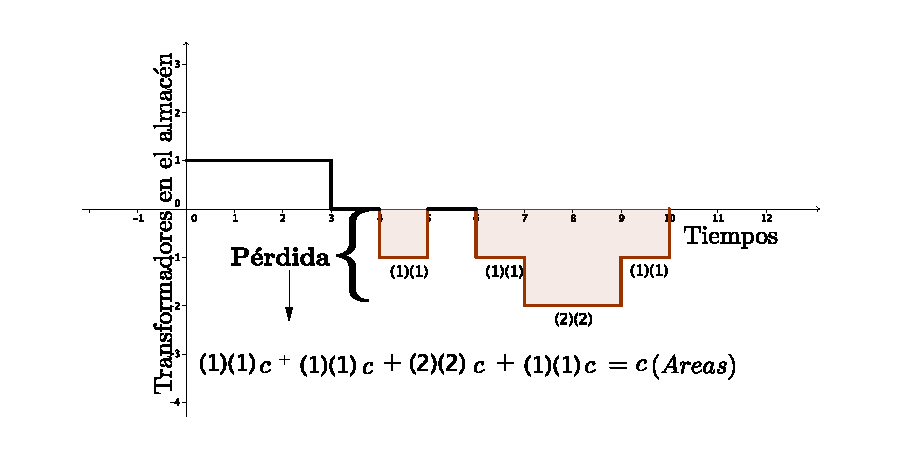
\includegraphics[scale=1]{tr1.pdf}
\end{center}
\vspace{-1.5 cm} \caption{\bf Almacenamiento de transformadores, hasta $10$ unidades de tiempo, mostrando la p\'erdida sobre ese per\'iodo.}\label{tr}
\end{figure}



\noindent De manera  general, podemos construir la funci\'on de p\'erdida asociada a la pol\'itica A, como se describe a continuaci\'on.\\[0.2cm]
\noindent Sean $\underline{T}=\{t_1,t_2,\cdots,t_n\}$ los tiempos de falla de los transformadores y 
$\underline{\ell}=\{\ell_1=t_1+\delta, \ell_2=t_2+\delta, \cdots, \ell_n=t_n+\delta\},$ los tiempos de llegada de los transformadores pedidos. 

\noindent  Definamos  $X(t;\underline{T})$ como el  n\'umero de transformadores en el almac\'en que se usaron para cubrir los tiempos de fallas hasta el tiempo $t$ y  $Y(t;\underline{T})$ el n\'umero de transformadores que se pidieron y llegaron antes del tiempo $t$. Luego $X(0)=n_0$ y $Y(0)=0$.\\[0.1cm]
\noindent Sea $Z(t,\underline{T})=X(t;\underline{T})+Y(t;\underline{T})$, indica el comportamiento de la funci\'on $n(t,n_0,\delta)$. Interesa conocer las veces en la cual esta permanece por debajo de cero.\\[0.1cm] 
\noindent La siguiente funci\'on restringue solo al \'area de inter\'es 
\[
W(t;\underline{T})=\left\{
\begin{array}{cl}
\displaystyle 0 & \mbox{ si } Z(t;\underline{T})\geq 0,\\                                                               Z(t)      &     \mbox{ si } Z(t;\underline{T})< 0  \\
\end{array}
\right.
\]

\noindent Una vez establecidas las funciones anteriores la funci\'on de p\'erdida esta dada por 

\begin{eqnarray}\label{LL}
L(t,\underline{T};\delta, n_0)=\int_{0}^{t} W(s;\underline{T}) ds,
\end{eqnarray}

\noindent dicho en palabras la p\'erdida esta representada por la integral sobre el periodo de observaci\'on, de las veces en las cuales el almac\'en se quedo sin transformadores disponibles para su uso.\\[0.1cm]
Para tener una idea clara de la forma de calcular (\ref{LL}), veamos el siguiente que ejemplo.\\[0.1cm]
 %Para $\underline{T}$, $Z(t)$ \\[0.2cm]


{\bf \noindent  Ejemplo:} 
\\[0.1cm]
Supongamos que en el intervalo $(0,7)$ de tiempo, ocurrieron solo 6 fallas, en los tiempos dados en la Tabla \ref{4500}. Es de inter\'es  conocer el n\'umero de transformadores al tiempo 7 con $n_0=3$ y $\delta=3$.
\begin{table}[h!]\small
\caption{\bf Valores de \underline{T}.\label{4500}}
\centering
\vspace{0.3cm }\begin{tabular}{cccccc}
\toprule[0.6mm]
0.730 & 0.812 & 0.868 &  2.786 &  3.064 &  3.401  \\
\toprule[0.6mm]
\end{tabular}
\end{table}


\noindent La Figura \ref{ejeu1} muestra dos gr\'aficas, la primera de lado izquierdo, ilustra a trav\'es del tiempo la forma de comportarse del n\'umero de  transformadores que se usaron para cubrir los tiempos de falla. Por cada tiempo de falla, el n\'umero de transformadores en el almac\'en disminuye en 1. Dado que iniciamos con 3 transformadores $X(0)=3$, al final de la sexta  falla $X(3.401)=-3$. 




\begin{figure}[h!]
\begin{center}
\includegraphics[scale=.35]{ejeu1.pdf}
\end{center}
\vspace{-1 cm} \caption {\bf Izquierda: Funci\'on $X(t)$ el n\'umero de transformadores en el almac\'en que se usaron para cubrir las fallas durante el periodo de observaci\'on. Derecha: Funci\'on $Y(t)$, describe los tiempos en que llegaron los transformadores que fueron solicitados.}\label{ejeu1}
\end{figure}

\noindent Mientras que del lado derecho vemos el comportamiento de $Y(t)$. Al tiempo cero, $Y(0)=0,$ ya que  no se ha pedido ning\'un transformador. La primera llegada ocurrir\'a al tiempo $t_1+\delta=0.730+3=3.730$, de ah\'i subir\'a cada $t_i+\delta$, donde los $t_i$'s son tomados de la Tabla \ref{4500}.  La  Tabla  \ref{23} muestra los tiempos en los cuales llegaron los transformadores pedidos.
\begin{table}[h!]\small
\centering
\caption{\bf Valores de $\underline{\ell.}$}\label{23}
\vspace{0.3cm }\begin{tabular}{cccccc}
\toprule[0.6mm]
3.730 & 3.812 & 3.868 &  5.786 &  6.064 &  6.401  \\
\toprule[0.6mm]
\end{tabular}

\end{table}



 \noindent Una vez teniendo estas gr\'aficas podemos obtener $Z(t)$ como la suma de ellas, mostrada en la Figura \ref{ejeu2}, esta gr\'afica representa los tiempos a los cuales fallaron los transformadores y llegaron los repuestos, de acuerdo a las Tablas \ref{4500} y \ref{23}. 

\begin{figure}[h!]
\begin{center}
\includegraphics[scale=.3]{ejeu2.pdf}
\end{center}
\vspace{-1 cm} \caption{\bf Funci\'on $Z(t)$ es el n\'umero de transformadores el almac\'en hasta $t=7.$}\label{ejeu2}
\end{figure}

\noindent El tiempo de permanencia sin transformadores y durante que periodos se observa en la Figura \ref{ejeu3},  representada por la funci\'on $W(t)$. Esta funci\'on es escalonada baja y sube seg\'un fue un tiempo de falla o un tiempo de llegada de un transformador pedido. Los valores expl\'icitos de $W(t)$, est\'an en la Tabla \ref{dosa}.

 
 
 \begin{figure}[h!]
\begin{center}
\includegraphics[scale=.3]{ejeu3.pdf}
\end{center}
\vspace{-1 cm}\caption{\bf Funci\'on $W(t)$ que representa la trayectoria negativa de los transformadores en el almac\'en.}\label{ejeu3}
\end{figure}


 
\begin{table}[h!]\small
\centering
\caption{\bf Valores de la funci\'on $W(t)$.}\label{dosa}
\begin{tabular}{ccccccc}
\toprule[0.6mm]
Tiempos&0.730& 0.812 & 0.868 &  2.786 &  3.064&  3.401  \\\hline
$W$(Tiempos) & 0  &0      &  0     & -1 &-2  &-3 \\
\hline
Tiempos&3.730 & 3.812 & 3.868 &  5.786 &  6.064&  6.401  \\\hline
$W$(Tiempos) & -2  &-1    &  0     & 0 &0  &0 \\
\toprule[0.6mm]
\end{tabular}

\end{table}

\newpage
 
\noindent  La funci\'on de p\'erdida dada en la Ecuaci\'on (\ref{LL}), se obtiene como el \'area de la funci\'on $W(t)$.

\begin{eqnarray*} 
L(\underline{T},3,3)&=&\int W(s) ds\\
&=& 1( 3.064-2.786)+ 2(3.401-3.064)+3(3.730- 3.401)\\
&+&2( 3.812- 3.730)+ 1(3.868-3.812)\\
&=&8.159
\end{eqnarray*}

\noindent Por lo tanto el valor de la funci\'on de p\'erdida es $8.159$.

\subsubsection{P\'erdida Esperada}

\noindent La funci\'on de p\'erdida dada por la Ecuaci\'on (\ref{LL}), depende de $n_0$, $\delta$ que son valores constantes y de \underline{T} que es una variable aleatoria, por lo tanto la funci\'on de p\'erdida es una funci\'on estoc\'astica, en el sentido de que depende de una variable aleatoria. Entonces la p\'erdida esperada tambi\'en es una funci\'on estoc\'astica, y esta dada por:
\begin{eqnarray}\label{ut}
U(t,n_0,\delta)=E(L(t,\underline{T},n_0, \delta)).
\end{eqnarray}

\noindent Por la ley de los grandes n\'umeros, la manera de estimar la Ecuaci\'on (\ref{ut}), es mediante la  expresi\'on:

\begin{eqnarray}\label{utqq}
\hat{U}(t,n_0,\delta)=\frac{1}{M} \sum_{s=1}^{M}\int_{0}^{t} W(y,\underline{T}_s) dy,
\end{eqnarray}
 donde $M$ es el n\'umero de $\underline{T}_s$ simulados.
\noindent Para calcular la expresi\'on (\ref{utqq}) por simulaci\'on se hace de la siguiente manera:

\begin{enumerate}
\item Se simulan $M$ trayectorias de tiempos de vida, dicho en otras palabras $M$ vectores del tipo $\underline{T}$.
\item Para cada trayectoria se calcula la Ecuaci\'on (\ref{LL}).
%que indica la p\'erdida en toda la trayectoria de tiempos simulada.
\item De los $M$ valores obtenidos,  se obtiene el promedio de ellos, que ser\'a la p\'erdida esperada.
%\item Una vez que se tienen las $M$, trayectorias y sus sumas asociadas, se calcula el promedio de las sumas, los cuales representan la p\'erdida esperada (Ecuaci\'on \ref{utqq}).\\[0.2cm]
\end{enumerate}

\noindent De acuerdo a los pasos anteriores, se realizaron 1000 simulaciones para cada pareja $$(\delta_i,n_{0_j})$$ donde $\delta_i=6, 8$ y 12 meses, $n_{0_j}=1,2,\cdots, 24$ que representa el n\'umero de transformadores al inicio del periodo. Luego se obtuvo el promedio de las funciones de p\'erdida, calculadas en cada una de las 1000 simulaciones para cada pareja, se consider\'o un tiempo de observaci\'on de 40 a\~nos (480 meses).\\[0.1cm]

\noindent La Figura \ref{d6s} muestra la gr\'afica de las p\'erdidas esperadas para $\delta=6,8,12$ meses.  Observamos que para valores de $n_0$ peque\~nos, 
las perdidas esperadas son grandes. A medida que $n_0$ crece, los promedios disminuyen. Al considerarse tiempos de espera m\'as largos, los costos tambi\'en se incrementan, las mayores p\'erdidas se tienen cuando $\delta=12$, para este periodo de espera se necesitan al menos 24 transformadores al inicio del periodo de observaci\'on (Tabla \ref{c777}). Para $\delta=8$ se requieren 15 transformadores (Tabla  \ref{c33333} )y para $\delta=6$ se necesitan 15 transformadores en el almac\'en (Tabla \ref{c1}).



\begin{figure}[h!]
\begin{center}
\includegraphics[scale=0.35]{poA.pdf}
\end{center}
\vspace{-1 cm} \caption{\bf P\'erdidas Esperadas con la Pol\'itica A, usando $t=480$, $\delta=6,8,12$ y Differentes Valores de $n_0$.}\label{d6s}
\end{figure}


%\begin{figure}[h!]
%\begin{center}
%\includegraphics[scale=0.25]{u6.pdf}
%\end{center}
%\vspace{-1 cm} \caption{\bf  p\'erdidaes esperadas con la pol\'itica A usando $t=480$ y $\delta=6$}\label{d6s}
%\end{figure}

\begin{table}[h!]\small
\centering
\caption{\bf Pol\'itica A: Valores de las P\'erdidas Esperadas con $\delta=6$.}\label{c1}
\vspace{0.3 cm}\begin{tabular}{ccccccccc}
\toprule[0.6mm]

$\bf{n_0}$&\bf{1} &                   \bf{2} &                   \bf{3} &                   \bf{ 4 }&                    \bf{ 5}&              \bf{ 6} &               \bf{ 7} & \bf{8} \\
\hline
$\mbox{\bf Promedio}$&1029.433  &697.822&  437.725&  251.263 & 131.085 &  62.514 &  27.148 &  11.136 \\	
\hline
$\bf{n_0}$&\bf{9} &                \bf{ 10}&              \bf{      11} &                   \bf{ 12} &               \bf{      13}&              \bf{14} &  \bf{ 15} & \bf{16 }   \\
\hline
$\mbox{\bf Promedio}$&	 4.003  &  1.343 &   0.446 &   0.167&    0.028 &   0.040 &   0.000&    0.000\\ 
	 \hline
	
$\bf{n_0}$&\bf{17} &     \bf{ 18}&   \bf{19}&   \bf{ 20} &           \bf{   21}&                \bf{  22}  & \bf{23} & \bf{24}  \\
\hline
$\mbox{\bf Promedio}$&  0.000 &   0.000&    0.000 &   0.000   & 0.000  &  0.000 &   0.000 & 0.000\\
\toprule[0.6mm]
\end{tabular}

\end{table}
%------------------------------------------------------------------------------------------------------------------------------------------------------------
%delta=7

%\begin{figure}
%\begin{center}
%\includegraphics[width=9cm,height=5cm]{delta7t480sumas.pdf}
%\end{center}
%\vspace{0.01 cm} \textsl{\caption{$n_0$ toma valores de 1 hasta 23, $t=480$ y $\delta=7$}\label{d7s}}
%\end{figure}
%
%
%\begin{table}[h!]
%\centering
%\begin{tabular}{|c|c|c|c|c|c|c|c|c|}
%\hline
%$\bf{n_0}$&\bf{1} &                   \bf{2} &                   \bf{3} &                   \bf{ 4 }&                    \bf{ 5}&              \bf{ 6} &               \bf{ 7} & \bf{8} \\
%\hline
%$Promedio$&1253.239 & 899.652 & 609.664 & 385.596&  223.191&  118.834 &  59.093  & 26.753\\ 
%\hline
%$\bf{n_0}$&\bf{9} &                \bf{ 10}&              \bf{      11} &                   \bf{ 12} &               \bf{      13}&              \bf{14} &  \bf{ 15} & \bf{16 }   \\
%\hline
%$Promedio$&	  10.901  &  4.472&    1.427 &   0.603  &  0.151 &   0.069&    0.012 &   0.000 \\
%	 \hline
%	
%$\bf{n_0}$&\bf{17} &     \bf{ 18}&   \bf{19}&   \bf{ 20} &           \bf{   21}&                \bf{  22}  & \bf{23} &  \\
%\hline
%$Promedio$&   0.000 &   0.000&    0.000 &   0.000   & 0.000  &  0.000 &   0.000 & \\
%   \hline
%\end{tabular}
%\caption{Valores obtenidos con $\delta=7$.}\label{c2}
%\end{table}
%
%
%
%-------------------------------------------------------------------------------------------------------------------------------------------------------------
%Delta=8

%\begin{figure}[h!]
%\begin{center}
%\includegraphics[scale=0.25]{u8.pdf}
%\end{center}
%\vspace{-1 cm} \caption{\bf p\'erdidaes esperadas con la pol\'itica A, usando $t=480$ y $\delta=8$}\label{d8ssss}
%\end{figure}


\begin{table}[h!]\small
\centering
\caption{\bf Pol\'itica A: Valores de las P\'erdidas Esperadas con $\delta=8$.}\label{c33333}
\vspace{0.3 cm}\begin{tabular}{ccccccccc}
\toprule[0.6mm]
$\bf{n_0}$&\bf{1} &                   \bf{2} &                   \bf{3} &                   \bf{ 4 }&                    \bf{ 5}&              \bf{ 6} &               \bf{ 7} & \bf{8} \\
\hline
$\mbox{\bf Promedio}$&1483.721 &1118.711  &799.610  &539.082 & 338.785  &200.591  &109.192  & 55.774 \\
\hline
$\bf{n_0}$&\bf{9} &                \bf{ 10}&              \bf{      11} &                   \bf{ 12} &               \bf{      13}&              \bf{14} &  \bf{ 15} & \bf{16 }   \\
\hline
$\mbox{\bf Promedio}$&	   25.935  & 11.184  &  4.376  &  1.637   & 0.733   & 0.219   & 0.081  &  0.032  \\
	 \hline
	
$\bf{n_0}$&\bf{17} &     \bf{ 18}&   \bf{19}&   \bf{ 20} &           \bf{   21}&                \bf{  22}  & \bf{23} & \bf{24}  \\
\hline
$\mbox{\bf Promedio}$&   0.004 &   0.003&    0.000 &   0.000   & 0.000  &  0.000 &   0.000 & 0.00\\
\toprule[0.6mm]
\end{tabular}

\end{table}
%----------------------------------------------------------------------------------------------------------------------------------------------------------


%Delta=9
%
%\begin{figure}
%\begin{center}
%\includegraphics[width=9cm,height=5cm]{delta9sumas.pdf}
%\end{center}
%\vspace{0.01 cm} \textsl{\caption{$n_0$ toma valores de 1 hasta 23, $t=480$ y $\delta=9$}\label{d9s}}
%
%\end{figure}
%
%\newpage
%
%
%\begin{table}[h!]
%\centering
%\begin{tabular}{|c|c|c|c|c|c|c|c|c|}
%\hline
%$\bf{n_0}$&\bf{1} &                   \bf{2} &                   \bf{3} &                   \bf{ 4 }&                    \bf{ 5}&              \bf{ 6} &               \bf{ 7} & \bf{8} \\
%\hline
%$Promedio$&1712.065 &1336.411 &1002.302  &713.153 & 478.761  &305.225 & 182.174 & 102.668  \\
%\hline
%$\bf{n_0}$&\bf{9} &                \bf{ 10}&              \bf{      11} &                   \bf{ 12} &               \bf{      13}&              \bf{14} &  \bf{ 15} & \bf{16 }   \\
%\hline
%$Promedio$&	   51.848 &  24.706  & 10.936 &   4.594 &   1.861 &   0.721   & 0.218   & 0.072   \\
%	 \hline
%	
%$\bf{n_0}$&\bf{17} &     \bf{ 18}&   \bf{19}&   \bf{ 20} &           \bf{   21}&                \bf{  22}  & \bf{23} &  \\
%\hline
%  $Promedio$& 0.039 &   0.010&    0.002 &   0.000   & 0.000  &  0.000 &   0.000 & \\
%   \hline
%\end{tabular}
%\caption{Valores obtenidos con $\delta=9$.}\label{c4}
%\end{table}
%
%%----------------------------------------------------------------------------------------------------------------------------------------------------------
%%Delta=10
%
%\begin{figure}
%\begin{center}
%\includegraphics[width=9cm,height=5cm]{delta10sumas.pdf}
%\end{center}
%\vspace{0.01 cm} \textsl{\caption{$n_0$ toma valores de 1 hasta 23, $t=480$ y $\delta=10$}\label{d10s}}
%
%\end{figure}
%\newpage
%
%\begin{table}[h!]
%\centering
%\begin{tabular}{|c|c|c|c|c|c|c|c|c|}
%\hline
%$\bf{n_0}$&\bf{1} &                   \bf{2} &                   \bf{3} &                   \bf{ 4 }&                    \bf{ 5}&              \bf{ 6} &               \bf{ 7} & \bf{8} \\
%\hline
%$Promedio$&1944.634 & 1560.876 &1210.653 &  905.893  & 642.491 &  436.292 &  273.966  &  167.279  \\
%\hline
%$\bf{n_0}$&\bf{9} &                \bf{ 10}&              \bf{      11} &                   \bf{ 12} &               \bf{      13}&              \bf{14} &  \bf{ 15} & \bf{16 }   \\
%\hline
%$Promedio$&	   91.176  &  48.178 &  23.693 &  11.076  &  4.752 &   2.030 &   0.759 &   0.400   \\
%	 \hline
%	
%$\bf{n_0}$&\bf{17} &     \bf{ 18}&   \bf{19}&   \bf{ 20} &           \bf{   21}&                \bf{  22}  & \bf{23} &  \\
%\hline
% $Promedio$&  0.069 &   0.026&    0.006 &   0.000   & 0.000  &  0.001 &   0.000 & \\
%   \hline
%\end{tabular}
%\caption{Valores obtenidos con $\delta=10$.}\label{c5}
%\end{table}
%%-----------------------------------------------------------------------------------------------------------------------------------------------------------
%%Delta=11
%
%\begin{figure}
%\begin{center}
%\includegraphics[width=9cm,height=5cm]{delta11sumas.pdf}
%\end{center}
%\vspace{0.01 cm} \textsl{\caption{$n_0$ toma valores de 1 hasta 23, $t=480$ y $\delta=11$}\label{d11s}}
%\end{figure}
%\newpage
%\begin{table}[h!]
%\centering
%\begin{tabular}{|c|c|c|c|c|c|c|c|c|}
%\hline
%$\bf{n_0}$&\bf{1} &                   \bf{2} &                   \bf{3} &                   \bf{ 4 }&                    \bf{ 5}&              \bf{ 6} &               \bf{ 7} & \bf{8} \\
%\hline
%$Promedio$&2173.671 &1781.718& 1427.693 &1098.406  &  819.975  & 583.561  &391.518 & 248.187   \\
%\hline
%$\bf{n_0}$&\bf{9} &                \bf{ 10}&              \bf{      11} &                   \bf{ 12} &               \bf{      13}&              \bf{14} &  \bf{ 15} & \bf{16 }   \\
%\hline
%$Promedio$&	151.415 &  84.731 &  46.088 &  23.408 &  10.532 &   5.272 &   2.169 &   0.823    \\
%	 \hline
%	
%$\bf{n_0}$&\bf{17} &     \bf{ 18}&   \bf{19}&   \bf{ 20} &           \bf{   21}&                \bf{  22}  & \bf{23} &  \\
%\hline
%$Promedio$&    0.325 &   0.093  &  0.055 &   0.011  & 0.000  &  0.001 &   0.000 & \\
%   \hline
%\end{tabular}
%\caption{Valores obtenidos con $\delta=11$.}\label{c6}
%\end{table}
%
%
%%-----------------------------------------------------------------------------------------------------------------------------------------------------------
%Delta=12
%\begin{figure}[h!]\small
%\begin{center}
%\includegraphics[scale=0.25]{u12.pdf}
%\end{center}
%\vspace{-1 cm}\caption{\bf p\'erdidaes esperadas con la pol\'itica A usando $t=480$ y $\delta=12$}\label{d12s}

%\end{figure}

\begin{table}[h!]\small
\centering
\caption{\bf Pol\'itica A: Valores de las P\'erdidas Esperadas con $\delta=12$.}\label{c777}
\vspace{.3cm}\begin{tabular}{ccccccccc}
\toprule[0.6mm]
$\bf{n_0}$ &\bf{1} &                   \bf{2} &                   \bf{3} &                   \bf{ 4 }&                    \bf{ 5}&              \bf{ 6} &               \bf{ 7} & \bf{8} \\
\hline
{\bf Promedio} & 2411.0  & 2008.7 &1640.9 &1305.0&1002.0 & 740.5 & 526.5 & 357.3    \\
\hline
$\bf{n_0}$&\bf{9} &                \bf{ 10}&              \bf{      11} &                   \bf{ 12} &               \bf{      13}&              \bf{14} &  \bf{ 15} & \bf{16 }   \\
\hline
{\bf Promedio}&	 222.7 & 137.1 &  78.0 &   41.8 &  21.1  &   9.8  &    4.8  &  2.3    \\
	 \hline
	
$\bf{n_0}$&\bf{17} &     \bf{ 18}&   \bf{19}&   \bf{ 20} &           \bf{   21}&                \bf{  22}  & \bf{23} &\bf {24}  \\
\hline
   {\bf Promedio} &  0.9    &  0.34 &   0.09 &   0.03 &   0.01 &   0.02 &   0.003  & 0.00\\
\toprule[0.6mm]
\end{tabular}

\end{table}
%------------------------------------------------------------------------------------------------------------------------------------------------------------
\newpage
\noindent Cabe destacar que los valores considerandos de $\delta$'s y $t=480$ meses, se utilizaron para  ilustrar la metodolog\'ia sugerida, puesto que no se tiene acceso a los valores reales. Sin embargo con la metodolog\'ia propuesta, cualesquiera que fueran los valores reales, los c\'alculos anteriores pueden realizarse.
%Es importante recalcar que la funci\'on de p\'erdida descrita en esta secci\'on, solo considera el costo que implica la falta de transformadores en el almac\'en.

%##########costo agregado#########

\subsection{Pol\'itica B}
\noindent Dentro de esta secci\'on se emplea la pol\'itica B, para establecer la funci\'on de p\'erdida utilizando los siguientes costos:

\begin{description}

\item [Costo 1:] \hfill \\El costo de no poder cobrar la electricidad durante un  periodo de tiempo donde no hab\'ia transformadores en reserva, considerado en la secci\'on anterior.
\item [Costo 2:] \hfill\\El costo de almacenamiento por unidad e de tiempo.
\end{description}

\noindent Sea $C$ el costo de no poder cobrar la electricidad en una unidad de tiempo. Luego el costo de almacenar un transformador por una unidad de tiempo, lo podemos expresar en t\'erminos de $C$ como
 $rC$. Asumiendo que el {\bf Costo 1} es mayor que el {\bf Costo 2} entonces $r \in(0,1)$.\\[0.1cm]
 
 
 
\noindent  La funci\'on de p\'erdida considerando el {\bf costo 1} y el costo inicial de almacenamiento durante la primera unidad de tiempo es:
\begin{eqnarray*}
L(t,\underline{T},\delta, n_0)=C\int_{0}^{t} W(s;\underline{T})  ds + rn_0C \mbox{ },
\end{eqnarray*}

\noindent Suponiendo $C=1$, es decir, una unidad de dinero. La p\'erdida  se simplifica a: 
\begin{eqnarray}\label{LL1}
L(t,\underline{T},\delta, n_0)=\int_{0}^{t} W(s;\underline{T})  ds + rn_0,
\end{eqnarray}
La p\'erdida esperada puede calcularse como:
\begin{eqnarray*}
\hat{U}(t,n_0,\delta)=\frac{1}{M} \sum_{s=1}^{M}\left(\int_{0}^{t} W(y;\underline{T}_s) dy + n_0r\right)
\end{eqnarray*}


 \noindent donde $M$ es el n\'umero de $\underline{T}$'s simulados. Es decir, a la p\'erdida  planteada en la secci\'on anterior se le suma la recta $rn_0$, como funci\'on de $n_0$. Esta recta representa los costos de almacenamiento de los transformadores inciales.
%Hemos entonces construido una nueva funci\'on de p\'erdida que considere las dos p\'erdidas, de tener almacenados transformadores extras y el costo de quedarnos sin ellos.\\[0.2cm]

\noindent Asignando valores a $r$, se puede observar la manera de comportarse de esta funci\'on de p\'erdida  (\ref{LL1}) y los valores de $n_0$'s que esta funci\'on proporcione. La manera de estimar la p\'erdida esperada es por medio de simulaciones (como se describe en la pol\'itica A). 
A continuaci\'on se muestran los resultados.\\[.2cm]
\noindent En la Figura \ref{u01p6} observamos las p\'erdidas esperadas suponiendo distintos n\'umeros de transformadores iniciales, y $r=0.1$, la recta mostrada corresponde a $n_0r$. A partir de cierto punto la p\'erdida esperada esta sobre la misma linea que la recta, esto indica que a partir del primer punto en el cual se da este parecido, la p\'erdida esperada se ve afectada por los costo de almacenamiento. 


\noindent En la Tabla \ref{r11} mostramos los valores graficados de la Figura \ref{u01p6}. De $n_0=1$ hasta 13, la p\'erdida esperada decrece, a partir de $n_0=13$ la p\'erdida empieza a crecer lentamente. Por lo que el $n_0$ \'optimo para $\delta=6$ meses y $r=0.1$ es 13 transformadores. Un comportamiento similar se observa en el resto de las Figuras mostradas (\ref{fi} y \ref{r0.5delta6}.
%%%%%%%%%%%%%%%%%#########################
%Delta=6

\begin{figure}[h!]
\begin{center}
\includegraphics[scale=0.3]{utilpeso01delta61.pdf}
\end{center}
\vspace{-1 cm}\caption{\bf P\'erdidas Esperadas con la Pol\'itica B, usando $\delta=6$ y r=0.1}\label{u01p6}
\end{figure}

\begin{table}[h!]\small
\centering
\caption{\bf Pol\'itica B: Valores de las P\'erdida  Esperadas con $\delta=6$, $r=0.1$.}\label{r11}
\begin{tabular}{ccccccccc}
\toprule[0.6mm]
$\bf{n_0}$ &\bf{1} &                   \bf{2} &                   \bf{3} &                   \bf{ 4 }&                    \bf{ 5}&              \bf{ 6} &               \bf{ 7} & \bf{8} \\
\hline
${\bf Promedio}$ &  
 1026.86 &  701.26 & 441.20 & 248.58 & 132.61  & 61.29 &  27.04&   12.30 \\
\hline
$\bf{n_0}$& \bf{9} &                \bf{ 10}&              \bf{      11} &                   \bf{ 12} &               \bf{      13}&              \bf{14} &  \bf{ 15} & \bf{16 }   \\
\hline
${\bf Promedio}$&	  5.50 &   2.71 &   1.50 &   1.39 &   1.34 &   1.43  &  1.50 &   1.60    \\
	 \hline
	
$\bf{n_0}$&\bf{17} &     \bf{ 18}&   \bf{19}&   \bf{ 20} &           \bf{   21}&                \bf{  22}  & \bf{23} & \bf{23}  \\
\hline
${\bf Promedio}$&    1.70  &1.80 &   1.90 &   2.00  &  2.10  &  2.20 &   2.30  &   2.40 \\
\toprule[0.6mm]
\end{tabular}

\end{table}





 
%%%%%%%%%%%%%%%%%%%%%%%%%%%%%%%%%%%

\noindent Para un periodo de reemplazo $\delta$=8 meses, los resultados de la p\'erdida  esperada se ven en la Figura \ref{fi} y los valores graficados en la Tabla \ref{r12}. A partir de $n_0=14$ la p\'erdida  esperada empieza a crecer.
%delta8
%t=480 siempre!!!!!!!!!!!!!
\begin{figure}[h!]
\begin{center}
\includegraphics[scale=0.3]{utilpeso01delta8.pdf}
\end{center}

\vspace{-1 cm}\caption{\bf P\'erdidas Esperadas con la Pol\'itica B, usando $\delta=8$ y r=0.1}\label{fi}
\end{figure}
\begin{table}[h!]\small
\centering
\caption{\bf Pol\'itica B: Valores de las P\'erdidas Esperadas con $\delta=8$, $r=0.1$.}\label{r12}
\begin{tabular}{ccccccccc}
\toprule[0.6mm]
$\bf{n_0}$ &\bf{1} &                   \bf{2} &                   \bf{3} &                   \bf{ 4 }&                    \bf{ 5}&              \bf{ 6} &               \bf{ 7} & \bf{8} \\
\hline
${\bf Promedio}$ & 1485.90 &1127.06 & 798.25  &545.79 & 347.76 & 205.38 & 114.38 &  56.49  \\
\hline
$\bf{n_0}$&\bf{9} &                \bf{ 10}&              \bf{      11} &                   \bf{ 12} &               \bf{      13}&              \bf{14} &  \bf{ 15} & \bf{16 }   \\
\hline
${\bf Promedio}$&	27.63 &  12.22 &   6.74 &   3.51  &  2.11&    1.49 &   1.52 &   1.61 \\
	 \hline
	
$\bf{n_0}$&\bf{17} &     \bf{ 18}&   \bf{19}&   \bf{ 20} &           \bf{   21}&                \bf{  22}  & \bf{23} &\bf{24}  \\
\hline
${\bf Promedio}$ &  1.72 &  1.80  &  1.90 &   2.00   & 2.10   & 2.20 &   2.30 &  2.40  \\
\toprule[0.6mm]
\end{tabular}

\end{table}

%%%%%%%%%%%%%%%%%%%
%delta12

%En la Figura 
%\begin{figure}[h!]
%\begin{center}
%\includegraphics[scale=0.25]{utipeso01delta12.pdf}
%\end{center}
%\vspace{0.01 cm} \textsl{\caption{$n_0$ toma valores de 1 hasta 20, $t=480$, $\delta=12$ y r=0.1}\label{d8s}}
%\end{figure}
%\begin{table}\small
%\begin{tabular}{|c|c|c|c|c|c|c|c|c|}
%\hline
%$\bf{n_0}$ &\bf{1} &                   \bf{2} &                   \bf{3} &                   \bf{ 4 }&                    \bf{ 5}&              \bf{ 6} &               \bf{ 7} & \bf{8} \\
%\hline
%$Promedio$ & 2827.56    & 2399.70 &2016.36 &1635.17 &1309.67  & 1005.63  & 748.15 & 520.04  \\
%\hline
%$\bf{n_0}$&\bf{9} &                \bf{ 10}&              \bf{      11} &                   \bf{ 12} &               \bf{      13}&              \bf{14} &  \bf{ 15} & \bf{16 }   \\
%\hline
%$Promedio$&	353.28& 232.40  &140.82  &     86.96 &  44.39  & 25.82  & 13.87  &  6.12  \\
%	 \hline
%	
%$\bf{n_0}$&\bf{17} &     \bf{ 18}&   \bf{19}&   \bf{ 20} &           \bf{   21}&                \bf{  22}  & \bf{23}   \\
%\hline
%$Promedio$  &  3.77  &  2.93  &   2.09  &    1.95  &  2.10 &   2.00  & 2.10 \\
%   \hline
%\end{tabular}
%\caption{Valores obtenidos con $\delta=12$, $r=0.1$.}\label{c7}
%\end{table}
%
%%%%%%%%%%%%%%%%%%%%%%%%%%%%
\newpage
\noindent En la Figura \ref{r0.5delta6} se muestra la grafica de la p\'erdida esperada con $r=0.5$. De la Tabla \ref{tt7} se deduce que  el n\'umero de transformadores iniciales, adecuados en el almac\'en es $n_0=11$.
%delta6 peso=0.5
\begin{figure}[h!]
\begin{center}
\includegraphics[scale=0.3]{utipeso05delta6.pdf}
\end{center}
\vspace{-1 cm} \caption{\bf P\'erdidas Esperadas con la Pol\'itica B, usando $\delta=6$ y r=0.5}\label{r0.5delta6}
\end{figure}


\begin{table}\small
\centering
\caption{\bf Pol\'itica B. Valores de las P\'erdidas Esperadas con $\delta=6$, $r=0.5$.}\label{tt7}
\begin{tabular}{ccccccccc}
\toprule[0.6mm]
$\bf{n_0}$ &\bf{1} &                   \bf{2} &                   \bf{3} &                   \bf{ 4 }&                    \bf{ 5}&              \bf{ 6} &               \bf{ 7} & \bf{8} \\
\hline
{\bf Promedio} & 1030.57 & 699.97&  432.87 & 249.35 & 135.35  & 65.35 &  31.56 &  14.56  \\
\hline
$\bf{n_0}$&\bf{9} &                \bf{ 10}&              \bf{      11} &                   \bf{ 12} &               \bf{      13}&              \bf{14} &  \bf{ 15} & \bf{16 }   \\
\hline
{\bf Promedio}&	9.15 &   6.56 &   5.65  &  6.08  &  6.57 &   7.00  &  7.50 & 8.00  \\
	 \hline
	
$\bf{n_0}$&\bf{17} &     \bf{ 18}&   \bf{19}&   \bf{ 20} &           \bf{   21}&                \bf{  22}  & \bf{23} &  \bf{24}\\
\hline
{\bf Promedio} &    8.50 &   9.00  &  9.50  &  10.0 &  10.50 &  11.00  & 11.50& 12.00\\
\toprule[0.6mm]
\end{tabular}

\end{table}

 

  


 %\noindent Sin embargo para observa la manera de comportarse de la %p\'erdida esperada para valores de $r>1$, se presenta en la Figura \ref{ultima} el caso cuando $r=3$, vemos que a partir de $n_0=9$, la p\'erdida crece de acuerdo al peso asignado para los transformadores de mas que se ve reflejado en la recta trazada que corresponde a $rn_0$.
%%%%%%%%%%%%%%%%%%%%%%%%%%%%%%%%%%
%delta8 peso=0.5
%%%%%%%%%%%%%%%%%%%%%%%%%%%%%%%%%%
%\begin{figure}[h!]
%\begin{center}
%\includegraphics[scale=0.25]{utipeso05delta8.pdf}
%\end{center}
%\vspace{0.01 cm} \textsl{\caption{$n_0$ toma valores de 1 hasta 20, $t=480$, $\delta=8$ y r=0.5}\label{d8s}}
%\end{figure}
%
%
%\begin{table}[ht]\small
%\begin{center}
%\begin{tabular}{|c|c|c|c|c|c|c|c|c|}
%  \hline
%$\bf{n_0}$ & \bf{1} &                   \bf{2} &                   \bf{3} &                   \bf{ 4 }&                    \bf{ 5}&              \bf{ 6} &               \bf{ 7} & \bf{8}  \\ 
%  \hline
%$Promedio$  & 1905.53 & 1475.03 & 1118.15 & 792.81 & 542.52 & 344.87 & 200.02 & 112.93 \\ 
%    \hline
% $\bf{n_0} $& \bf{9} &                \bf{ 10}&              \bf{      11} &                   \bf{ 12} &               \bf{      13}&              \bf{14} &  \bf{ 15} & \bf{16 }   \\
%      \hline
%$Promedio$  & 59.50 & 28.95 & 16.54 & 10.58 & 7.10 & 7.24 & 7.22 & 7.63 \\ 
%        \hline
%$\bf{n_0}$& \bf{17} &     \bf{ 18}&   \bf{19}&   \bf{ 20} &           \bf{   21}&                \bf{  22}  & \bf{23} &\\
%   \hline
%$Promedio$  & 8.05 & 8.50 & 9.00 & 9.50 & 10.00 & 10.50 & 11.00 &\\
%   \hline
%\end{tabular}
%\end{center}
%\caption{Valores obtenidos con $\delta=8$, $r=0.5$.}\label{c7}
%\end{table}
%

%%%%%%%%%%%%%%%%%%%%%%%%%%%%%%%%%%
%%delta12 peso=0.5
%\begin{figure}[h!]
%\begin{center}
%\includegraphics[scale=0.25]{utipeso05delta12.pdf}
%\end{center}
%\vspace{0.01 cm} \textsl{\caption{$n_0$ toma valores de 1 hasta 20, $t=480$, $\delta=12$ y r=0.5}\label{d8s}}
%\end{figure}
%
%\begin{table}[ht]\small
%\begin{center}
%\begin{tabular}{|c|c|c|c|c|c|c|c|c|}
%  \hline
% $\bf{n_0}$ & \bf{1} &                   \bf{2} &                   \bf{3} &                   \bf{ 4 }&                    \bf{ 5}&              \bf{ 6} &               \bf{ 7} & \bf{8}  \\ 
%  \hline
% $Promedio$& 2836.83 & 2420.81 & 2005.58 & 1642.06 & 1330.67 & 1019.24 & 732.47 & 531.32 \\ 
%  \hline
%  $\bf{n_0} $& \bf{9} &                \bf{ 10}&              \bf{      11} &                   \bf{ 12} &               \bf{      13}&              \bf{14} &  \bf{ 15} & \bf{16 }   \\
%  \hline
%  
% $Promedio$ & 362.90 & 237.12 & 142.27 & 85.43 & 54.08 & 28.78 & 16.39 & 13.50 \\ \hline
%  $\bf{n_0}$& \bf{17} &     \bf{ 18}&   \bf{19}&   \bf{ 20} &           \bf{   21}&                \bf{  22}  & \bf{23} &\\
%   \hline
% $Promedio$ & 9.54 & 9.24 & 9.19 & 9.55 & 10.04 & 10.51 & 11.00 & \\ 
%   \hline
%\end{tabular}
%\end{center}
%\caption{Valores obtenidos con $\delta=12$, $r=0.5$.}\label{c7}
%\end{table}

%delta 6 peso 3
%\begin{figure}[h!]
%\begin{center}
%\includegraphics[scale=0.25]{utipeso3delta6.pdf}
%\end{center}
%\vspace{0.01 cm} \textsl{\caption{$n_0$ toma valores de 1 hasta 20, $t=480$, $\delta=6$ y r=3}\label{ultima}}
%\end{figure}

%
%%delta 8 peso 3
%\begin{figure}[h!]
%\begin{center}
%\includegraphics[scale=0.25]{utipeso3delta8.pdf}
%\end{center}
%\vspace{0.01 cm} \textsl{\caption{$n_0$ toma valores de 1 hasta 20, $t=480$, $\delta=8$ y r=3}\label{d8s}}
%\end{figure}
%
%%delta 12 peso 3
%\begin{figure}[h!]
%\begin{center}
%\includegraphics[scale=0.25]{utipeso3delta12.pdf}
%\end{center}
%\vspace{0.01 cm} \textsl{\caption{$n_0$ toma valores de 1 hasta 20, $t=480$, $\delta=12$ y r=3}\label{d8s}}
%\end{figure}

%\newpage \thispagestyle{empty} \cleardoublepage

\subsection{Pol\'itica C}
\noindent Esta \'ultima pol\'itica considera los dos costos empleados en la Pol\'itica B por unidad de tiempo. La funci\'on de p\'erdida, esta dada por la siguiente expresi\'on.


\begin{eqnarray}
L(t,\underline{T},\delta,n_0)=\int_{0}^{t} W(s,\underline{T}) ds + r \int_{0}^{t} A(s,\underline{T}) ds
\end{eqnarray}
donde:
\[
A(t,\underline{T})=\left\{
\begin{array}{cl}
\displaystyle 0 & \mbox{ si } Z(t,\underline{T})\leq 0,\\                                                               Z(t)      &     \mbox{ si } Z(t,\underline{T})>0  \\
\end{array}
\right.
\]

\noindent La funci\'on $A(t,\underline{T})$ refleja las p\'erdidas que existen por almacenar transformadores. Para este caso la p\'erdida esperada se calcula como:
\begin{eqnarray}\label{LL3}
\hat{U}(t,n_0,\delta)&=& \frac{1}{M}\sum_{s=1}^M \left(     \int_{0}^{t} W(s,\underline{T}) ds + r \int_{0}^{t} A(s,\underline{T}) ds       \right).
\end{eqnarray}

\noindent Para evaluar la Ecuaci\'on (\ref{LL3}) procedemos de la misma manera que en las pol\'iticas anteriores.  A continuaci\'on se mostraran algunas gr\'aficas (Figuras \ref{u38i} y \ref{u36i}) y Tablas  (\ref{u38t} y \ref{u36t}) de los resultados.

\begin{figure}[h!]
\begin{center}
\includegraphics[scale=0.3]{uA8.pdf}
\end{center}
\vspace{-1 cm} \caption{\bf P\'erdidas Esperadas con la Pol\'itica C, usando $\delta=6$ y $r=0.01$}\label{u38i}
\end{figure}


\begin{table}[h!]\small
\centering
\caption{\bf Pol\'itica C. Valores de las P\'erdidas Esperadas con $\delta=6$ y $r=0.01$.}\label{u38t}
\begin{tabular}{ccccccccc}
\toprule[0.6mm]
$\bf{n_0}$&\bf{1} &                   \bf{2} &                   \bf{3} &                   \bf{ 4 }&                    \bf{ 5}&              \bf{ 6} &               \bf{ 7} & \bf{8} \\
\hline
{\bf Promedio}& 611687.9 &413680.9 &256825.8& 150424.5&  75977.0  &37610.2 & 16419.3 &   6576.2  \\
\hline
$\bf{n_0}$&\bf{9} &                \bf{ 10}&              \bf{      11} &                   \bf{ 12} &               \bf{      13}&              \bf{14} &  \bf{ 15} & \bf{16 }   \\
\hline
{\bf Promedio}&	    2408.7  & 1021.0 &   190.9 &   140.7 & 138.1  &  117.3  &  114.6 &   124.0  \\
	 \hline
	
$\bf{n_0}$&\bf{17} &     \bf{ 18}&   \bf{19}&   \bf{ 20} &           \bf{   21}&                \bf{  22}  & \bf{23} &  \bf{24}\\
\hline
{\bf Promedio}&  133.4 &   144.0 &152.2    &163.5 &   172.2  &  180.6 &   190.4 &199.2\\
\toprule[0.6mm]
\end{tabular}

\end{table}
%#---------------------------------------------------------------------------------------------------------------------------------------------------------%r=0.1
\begin{figure}[h!]
\begin{center}
\includegraphics[scale=0.3]{uA6puntouno.pdf}
\end{center}
\vspace{-1 cm} \caption{\bf P\'erdidas Esperadas con la Pol\'itica C, usando $\delta=6$ y $r=0.1$.}\label{u36i}
\end{figure}


\begin{table}[h!]\small
\centering
\caption{\bf Pol\'itica C: Valores de la P\'erdidas Esperadas con $\delta=6$ y $r=0.1$.}\label{u36t}
\begin{tabular}{ccccccccc}
\toprule[0.6mm]
$\bf{n_0}$&\bf{1} &                   \bf{2} &                   \bf{3} &                   \bf{ 4 }&                    \bf{ 5}&              \bf{ 6} &               \bf{ 7} & \bf{8} \\
\hline
{\bf Promedio}& 606757 & 417457 &258881& 151181 & 78446 & 38066 & 15675&  6799  \\
\hline
$\bf{n_0}$&\bf{9} &                \bf{ 10}&              \bf{      11} &                   \bf{ 12} &               \bf{      13}&              \bf{14} &  \bf{ 15} & \bf{16 }   \\
\hline
{\bf Promedio}&	    2385 &  1332&   563 &   526 &   566 &   576&  628  &  686   \\
	 \hline
	
$\bf{n_0}$&\bf{17} &     \bf{ 18}&   \bf{19}&   \bf{ 20} &           \bf{   21}&                \bf{  22}  & \bf{23} &  \bf{24}\\
\hline
{\bf Promedio}&   732  &  785 &  836&   889  &  941&  992 &  1046 &  1098\\
 \toprule[0.6mm]
\end{tabular}

\end{table}


%%%%%%%%%%%%%%%%%%%%%%%%%%%%%
%%r=0.1,delta=8 meses

%\begin{figure}[h!]
%\begin{center}
%\includegraphics[scale=0.25]{uA018.pdf}
%\end{center}
%\vspace{-1 cm} \caption{\bf P\'erdidas Esperadas con la Pol\'itica C, usando $\delta=8$ y $r=0.1$.}\label{u38ir}
%\end{figure}
%
%
%\begin{table}[h!]\small
%\centering
%\caption{\bf Pol\'itica C. Valores de las p\'erdidaes esperadas con $\delta=8$ y $r=0.1$.}\label{u38tt}
%\begin{tabular}{ccccccccc}
%\toprule[0.6mm]
%$\bf{n_0}$&\bf{1} &                   \bf{2} &                   \bf{3} &                   \bf{ 4 }&                    \bf{ 5}&              \bf{ 6} &               \bf{ 7} & \bf{8} \\
%\hline
%{\bf Promedio}&  879459  &664530& 473553&319889& 203962 &116103 & 65056  &31734 \\
%\hline
%$\bf{n_0}$&\bf{9} &                \bf{ 10}&              \bf{      11} &                   \bf{ 12} &               \bf{      13}&              \bf{14} &  \bf{ 15} & \bf{16 }   \\
%\hline
%{\bf Promedio}&	    16533  & 8093 & 3087 &  1483 &    803   & 675 &   606 &   678   \\
%	 \hline
%	
%$\bf{n_0}$&\bf{17} &     \bf{ 18}&   \bf{19}&   \bf{ 20} &           \bf{   21}&                \bf{  22}  & \bf{23} &  \bf{24}\\
%\hline
%{\bf Promedio}&   683  &  733 &  786 &   838 &   891  942  & 995   &1046&   1098  
%\\
%\toprule[0.6mm]
%\end{tabular}
%\end{table}
%
%%%%%%%%%%%%%%%%%%%%%%%%%%%
%
%r=0.5,delta=6 meses

\begin{figure}[h!]
\begin{center}
\includegraphics[scale=0.3]{puntocinco.pdf}
\end{center}
\vspace{-1 cm}\caption{\bf P\'erdidas Esperadas con la Pol\'itica C, usando $\delta=8$, $r=0.5$.}\label{u385i}
\end{figure}

%%
%%\begin{table}[h!]\small
%%\centering
%%\begin{tabular}{|c|c|c|c|c|c|c|c|c|}
%%\hline
%%$\bf{n_0}$&\bf{1} &                   \bf{2} &                   \bf{3} &                   \bf{ 4 }&                    \bf{ 5}&              \bf{ 6} &               \bf{ 7} & \bf{8} \\
%%\hline
%%$Promedio$&  877278 & 661102  &472981   & 326454 &205788 &119029 & 67981  &35501 \\
%%\hline
%%$\bf{n_0}$&\bf{9} &                \bf{ 10}&              \bf{      11} &                   \bf{ 12} &               \bf{      13}&              \bf{14} &  \bf{ 15} & \bf{16 }   \\
%%\hline
%%$Promedio$&	    877278 & 661102  &472981   &326454 &205788 &119029&67981  &35501   \\
%%	 \hline
%%	
%%$\bf{n_0}$&\bf{17} &     \bf{ 18}&   \bf{19}&   \bf{ 20} &           \bf{   21}&                \bf{  22}  & \bf{23} &  \bf{24}\\
%%\hline
%%$Promedio$&     3401 & 3645 &  3890&  4130&   4364  & 4611 &  4854 &  5094 
%%\\
%%   \hline
%%\end{tabular}
%%\caption{Valores obtenidos con $\delta=8$ y $r=0.5$.}\label{c333}
%%\end{table}
%
%
%%%%%%%%%%%%%%%%%%%%%%%%%%%
\noindent Las gr\'aficas presentadas tienen un comportamiento similar, a las que previamente ya hab\'iamos obtenido. La tendencia es bajar para los primeros valores de $n_0$ y posteriormente subir. La diferencia m\'as significativa radica en  el hecho de que los costos, a los cuales se minimiza $n_0$ son mucho mayores que en las anteriores funciones de p\'erdida. Este hecho se debe a que dentro de esta \'ultima pol\'itica se consideran costos de almacenamiento por cada unidad de tiempo.

\section{Conclusiones}
\noindent A lo largo de este cap\'itulo se han obtenido valores  para el n\'umero de transformadores iniciales que se deben de tener en el inventario. La Tablas  \ref{taba1},\ref{resu2} y \ref{resuFF},  resumen los valores obtenidos y mencionados en las secciones anteriores.
\begin{table}[h!]\small
\begin{center}
\caption{\bf Resultados de la Pol\'itica A.}\label{taba1}
\vspace{0.3cm}\begin{tabular}{ccc}
\toprule[0.6mm]
  $\delta$ & $n_0$ & costo\\
\toprule[0.6mm]
  6 & 15 &0.00\\
  8&19& 0.00\\
  12&24 & 0.00\\
\toprule[0.6mm]
\end{tabular}
\end{center}
%\caption{$n_0$'s \'optimos considerando solo el costo de quedarnos sin transformadores.}\label{resu1}
\end{table}

%\noindent En la Tabla \ref{taba1} se resumen los resultados obtenidos para los diferentes valores de $r$ y $\delta$, bajo la pol\'itica A. El n\'umero de transformadores \'optimos $n_0$ son menores que los presentados en la Tabla \ref{resu2}, pero los costos son mayores. Este hecho es producido al considerar los costos de almacenamiento por cada unidad de tiempo, es decir por cada mes, durante el periodo de observaci\'on (40 a\~nos). 
\noindent En la Tabla \ref{taba1} se muestran los valores \'optimos de transformadores iniciales que deben tenerse en el almac\'en, para un periodo de tiempo de $40$ a\~nos con diferentes valores de $\delta$, bajo la pol\'itica A. Es normal observar que entre mayor sea el periodo de espera de un transformador solicitado, mayor ser\'a el n\'umero de transformadores requeridos para el almacenamiento. Los costos asociados son cero, indica que a partir de la cantidad $n_0$ de transformadores, no habr\'a p\'erdidas en cuanto a la falta de ellos. Las conclusiones anteriores corresponden solo al considerarse un costo. Para ambos costos, los resultados se muestran en la Tabla \ref{resu2}, para diferentes valores de $r$ y usando la pol\'itica B.


\begin{table}[ht]\small
\begin{center}
\caption{\bf Resultados de la Pol\'itica B.}\label{resu2}
\vspace{0.3cm}\begin{tabular}{cccc}
\toprule[0.6mm]
 $\delta$ & $n_0$  & costo& $r$\\
\toprule[0.6mm]
  6   & 14 & 0.14& 0.01\\
  8   & 17 & 0.16& 0.01\\
  12 & 22  & 0.20 & 0.01\\
  \hline
  6   & 13 & 1.34& 0.1\\
  8   & 14 & 1.49& 0.1\\
  12 & 20 & 2.00& 0.1\\
  \hline
  6   & 11& 5.65 &0.5 \\
  8   & 14 &7.11 & 0.5 \\
  12 & 18 &9.16 &0.5\\
\toprule[0.6mm]
\end{tabular}
\end{center}

\end{table}






\noindent De la Tabla  \ref{resu2} notamos que al a\~nadir costos de almacenamiento inicial, los costos para $n_0$ obtenidos no se minimizan a cero.\\[0.1cm]
\noindent Cuando $r=0.01$, indica que si el costo de no tener un transformador disponible es $c$, entonces el costo por tener un transformador almacenado y no usarlo es $rc=\displaystyle\frac{1}{100}c$. El quedarse sin un transformador es 100 veces m\'as caro que almacenar un transformador y no usarlo. Para un periodo de espera $\delta=8$ meses se obtiene que  $n_0=17$ y el costo asociado es $0.16$. El valor de $n_0$ es menor que el obtenido en la Tabla \ref{taba1}, pero el costo es mayor. Esto se debe a que la funci\'on de p\'erdida dada por la Ecuaci\'on (\ref{LL1}), involucra costos de almacenamiento, entonces la p\'erdida esperada buscar\'a tener la m\'inima cantidad de transformadores al costo m\'as peque\~no posible. Los resultados obtenidos para $r=0.01$ no son tan significativamente variante de los mostrados en la Tabla \ref{taba1}, ya que la proporci\'on $r$, es peque\~na. Las diferencias notorias son para valores de $r$ mayores.\\[0.1cm]

\noindent Al tener $r=0.1$, indica que el quedarnos sin transformadores en 10 veces m\'as costoso que tener almacenados transformadores. Los costos a los cuales se minimiza la p\'erdida esperada oscilan de $1$ a $2$ unidades de $c$ y los valores de $n_0$ son menores o iguales al considerar solo la pol\'itica A. Un efecto similar ocurre al considerar $r=0.5$. \\[0.1cm]
 A medida que $r$ crece, el valor de $n_0$ se hace peque\~no y el costo aumenta. Entre mayor sea el costo de almacenamiento, se buscar\'a tener menos transformadores.\\[0.2cm]
Finalmente para la pol\'itica C, los costos aumentan significativamente respecto a la pol\'itica A y B. Ahora se consideran costos por unidad de tiempo, tanto de falta de ellos como de almacenamiento. As\'i que se busca no  tener transformadores en el almac\'en pero tampoco necesitarlos, raz\'on por la cual, los costos   de optimizaci\'on para esta pol\'itica son altos y los valores de $n_0$ asociados son menores a los de las pol\'iticas anteriores.
\begin{table}[h!]\small
\begin{center}
\caption{\bf Resultados de la Pol\'itica C.}\label{resuFF}
\vspace{0.3cm}\begin{tabular}{cccc}
\toprule[0.6mm]
 $\delta$ & $n_0$  & costo& $r$\\
\toprule[0.6mm]
  6   & 15 & 114& 0.01\\
  8   & 16 & 119& 0.01\\
  12 & 20  & 145 & 0.01\\
  \hline
  6   & 12 & 526& 0.1\\
  8   & 15 & 606& 0.1\\
  12 & 20 & 779& 0.1\\
  \hline
  6   & 11& 2209&0.5 \\
  8   & 14&2524 & 0.5 \\
  12 & 15 &8836 &0.5\\
\toprule[0.6mm]
\end{tabular}
\end{center}

\end{table}


\noindent Una vez presentadas las funciones  de p\'erdida planteadas y los resultados obtenidos. La pregunta de mayor inter\'es es ?`C\'ual es la m\'as adecuada?. La aplicaci\'on de cualquiera de ellas depender\'a de las condiciones reales del problema, determinadas por la empresa. Por ejemplo, si dentro la empresa, el principal costo a minimizar es el de no poder cobrar la electricidad, en el tiempo que no se tenga un transformador de reemplazo, entonces aplicar\'iamos la propuesta A. Si  por otra parte la empresa determina que adem\'as de considerar el costo de no tener transformadores disponibles, le  interesa minimizar el costo de almacenamiento $n_0$, al inicio de su periodo de observaci\'on, m\'as el costo de no tenerlos. Y justifica que a lo largo del tiempo el adquirir solo un transformador  a la vez no le afecta de manera significa, pero que el adquirir m\'as de uno, si representa gastos importantes, entonces ser\'ia adecuado considerar pol\'itica B. Finalmente si para la empresa los costo de almacenar y de no tener transformadores en reserva afectan de manera importante, emplear\'iamos la \'ultima funci\'on de p\'erdida propuesta. La aplicaci\'on de las pol\'iticas estar\'a ligada esencialmente a las necesidades de la empresa que se dedica a emplear como instrumentos de trabajo este tipo de transformadores. \\[0.2cm]
\noindent A lo largo de este cap\'itulo hemos planteado una manera de proponer una funci\'on, que cuantifique  la perdida esperada por la falta de transformadores en el almac\'en. Existen distintas formas de plantear el remplazamiento de los transformadores, inclusive otras funciones de p\'erdida podr\'ian ser exploradas. Sin embargo dentro del desarrollo de este trabajo se propuso una posible soluci\'on y se presentaron los resultados.



\newpage \thispagestyle{empty} \cleardoublepage

%\end{document}
